% Report on Predator-Prey Equations
% May 7, 2020, Moritz Konarski, AUCA

\newcommand{\name}{Moritz M. Konarski}
\newcommand{\datum}{\today}
\newcommand{\heading}{Predator-Prey Equations -- Modeling Food Chains}

\documentclass[12pt,a4paper,reqno]{amsart}

\usepackage[english]{babel}
\usepackage[utf8]{inputenc}
\usepackage{amsmath}
\usepackage{amsfonts}
\usepackage{anysize}
\usepackage{textcomp}
\usepackage{graphicx}
\graphicspath{{../graphics/}}
\usepackage{subfig}
\usepackage{wrapfig}
\usepackage{float}
\usepackage{fancyhdr}
\usepackage{lastpage}
\usepackage{caption}
\usepackage[dvipsnames]{xcolor}
\definecolor{magenta1}{rgb}{0, 0.35, 0.35}
\definecolor{green1}{rgb}{0, 0.45, 0}
\definecolor{red1}{rgb}{0.65, 0, 0}
\usepackage{hyperref}
\hypersetup{
    final,
    pdftitle={\heading},
    pdfauthor={\name},
    pdfsubject={Differential Equations},
    pdfkeywords={Predator-Prey Equations},
    breaklinks=true,
    colorlinks=true,
    citecolor=green1,
    urlcolor=magenta1,
    linkcolor=red1
}
\usepackage{calc}
\setlength{\footskip}{\paperheight
  -(1.25in+\voffset+\topmargin+\headheight+\headsep+\textheight)
  -1in}
\setlength{\headsep}{\voffset+\topmargin+\headheight + 0.4in}
\setlength{\parindent}{2em}
\setlength{\parskip}{2pt}
\renewcommand{\baselinestretch}{1.5}
\marginsize{1.25in}{1.25in}{0.9in}{1.5in}

\newcommand{\figref}[1]{\textsc{\figurename}~\ref{#1}}

\newcommand{\makefig}[4]{
\begin{figure}[#1]
    \captionsetup{justification=centering}
    \includegraphics[width=#2]{#3}
    \caption{#4}
    \label{fig:#3}
\end{figure}
}

\newcommand{\makewrapfig}[5]{
\begin{wrapfigure}{#1}{#2}
    \captionsetup{margin=10pt,justification=centering}
    \includegraphics[width=#3]{#4}
    \caption{#5}
    \label{fig:#4}
\end{wrapfigure}
}

\begin{document}
\begin{titlepage}
    \begin{center}
        \vspace*{1cm}
        \Huge
        \textbf{\heading{}\\}
        \vspace{0.5cm}
        \vspace{1.5cm}
        \LARGE
        \textbf{\name{}}
        \vfill
        \vspace{0.3cm}
        \Large
        Applied Mathematics Department,\\
        American University of Central Asia\\
        Bishkek, Kyrgyzstan\\
        \datum{}
    \end{center}
\end{titlepage}

\thispagestyle{plain}
\begin{center}
    \Large
    \textbf{\heading{}}\\
    \vspace{0.4cm}
    \large
    \textbf{\name{}}
    \vspace{0.6cm}
\end{center}
\textsc{Abstract.} This report covers models for two and three-species food
chains. The two-species food chain models covered by this report are made up of
a prey that lives off an infinite food supply and gets eaten by a predator that
exclusively eats this prey. The most well-known such model are the
Lotka-Volterra differential equations, named after the mathematicians that
discovered them. These equations can be extended to model a three-species food
chain where the predator from the two-species system is now preyed on by an
apex predator that exclusively eats that predator. This change makes the system
of differential equations more interesting to analyze. For this analysis the
mathematical software system SageMath will be used. Graphs and phase planes of
the discussed systems will be provided.

MSC: \textsc{34A01}

\vspace{-0.2\baselineskip}
\renewcommand{\baselinestretch}{1}
\tableofcontents
\renewcommand{\baselinestretch}{1.5}

\pagestyle{fancy}
\renewcommand{\headrulewidth}{0pt}
\fancyhead{}
\fancyhead[CE]{\textsc{\name{}}}
\fancyhead[CO]{\textsc{\heading{}}}
\newpage

%==============================================================================

\section{Introduction}

Predator-Prey equations are differential equations describing the populations
of predators and their prey. They describe the change in the number of
organisms depending on certain parameters. The most famous predator-prey
equations are the so-called Lotka-Volterra equations. They were derived
independently by Vito Volterra (1860--1940) and Alfred James Lotka (1880--1949)
in the 1920s \cite{hoppensteadt}.

Lotka (chemist, ecologist, mathematician) published his work on population
dynamics in 1925 on the basis of his earlier work with oscillating chemical
reactions in 1910 and 1920 where he derived the same equations \cite{israel}.
Volterra (mathematician, physicist) based his work on the number of predator
and prey fish in the Adriatic sea during WWI where he noticed a decrease in
prey and increase in predator fish \cite{hoppensteadt}. Both of their
approaches lead them to the same system of differential equations because the
processes they sought to describe are isomorphic -- they are non-linear
oscillators \cite{israel}. Thus the Lotka-Volterra equations describe any
process of two things changing and influencing each other -- plants getting
eaten by herbivores, parasites living off their hosts, or oscillating chemical
reactions \cite{hoppensteadt}.

%------------------------------------------------------------------------------

\subsection{Lotka-Volterra Equations}
Lotka-Volterra equations are the simplest predator prey equations
\cite{hoppensteadt}. They describe the development of two species over time
using continuous functions \cite{chauvet}, \cite{hoppensteadt}. Following
\cite{chauvet}, equation \eqref{eq:2s_system} shows the Lotka-Volterra system
of equations.
\begin{equation}    
    \left\{\begin{aligned}
        &\frac{dx}{dt} = ax - bxy \quad &\text{Prey}\\
        &\frac{dy}{dt} = -cy +dxy \quad &\text{Predator}
    \end{aligned}\right.
    \label{eq:2s_system}
\end{equation}
In \eqref{eq:2s_system}, $dx/dt$ is the change of the prey population, $dy/dt$
the change of the predator population. The constants $a,b,c,d > 0$ in this 
system of equations represent
\begin{itemize}
    \item $a$ -- growth rate of the prey if there are no predators,
    \item $b$ -- effect of predators killing prey,
    \item $c$ -- death rate of predators if there is no prey,
    \item $d$ -- growth rate of predators if there is prey \cite{chauvet}.
\end{itemize}

%------------------------------------------------------------------------------

\subsection{Expanded Lotka-Volterra Equations}
Equation \eqref{eq:2s_system} models a two-species food chain where $x$ is the
prey that gets eaten by $y$ which is above it in the food chain. This model can 
be extended to a three-species system that describes the populations of three
species part of the same food chain. Examples of these food chains are
mouse--snake--owl and vegetation--hare--lynx \cite{chauvet}. This expansion
requires a third equation to be added to our system. Again, following
\cite{chauvet}, we get equation \eqref{eq:3s_system}.
\begin{equation}
    \left\{\begin{aligned}
        &\frac{dx}{dt} = ax - bxy              &\text{Prey}\\
        &\frac{dy}{dt} = -cy + dxy - eyz \quad &\text{Intermediate Predator}\\
        &\frac{dz}{dt} = -fz + gyz             &\text{Apex Predator}
    \end{aligned}\right.
    \label{eq:3s_system}
\end{equation}
The above equation models a food chain where prey $x$ gets eaten by
intermediate predator $y$, which in turn gets eaten by apex predator $z$. Of
the constants $a,b,c,d,e,f,g > 0$, we have $a,b,c,d$ from \eqref{eq:2s_system}
which have the same functions. The remaining constants represent
\begin{itemize}
    \item $e$ -- effect of predator $z$ eating $y$,
    \item $f$ -- death rate of predator $z$ in absence of $y$,
    \item $g$ -- growth rate of predator $z$ if there is prey.
\end{itemize}
Equation \eqref{eq:3s_system} is a direct generalization of 
\eqref{eq:2s_system} which makes it both more interesting and more difficult to
solve \cite{chauvet}. Both two-species and three-species food chains will be
covered in this report.

%------------------------------------------------------------------------------

\subsection{Phase Planes}\label{sec:phase_plane}
Phase planes are a special form of state space, the set of all possible states
of a dynamic system. Every possible state of a system corresponds to a point in
state space \cite{terman}. For two-dimensional systems of autonomous 
(independent of time \cite{kreyszig}) ordinary differential equations, state
space is called a phase plane. In this phase plane the points representing
solutions to the system of equations move with time. Points moving over time
trace trajectories in the phase plane. If a point does not move in a phase
plane it is called equilibrium. If a point traces a closed trajectory the
solution represented by that point is periodic \cite{terman}. The movement of
a system in phase space is represented by vectors that show the velocity of
a system at that point.

In \figref{fig:example_phase_plane} we see the phase plane for a system of
differential
\makewrapfig{r}{0.65\textwidth}{0.65\textwidth}{example_phase_plane}{Phase
plane of a pendulum with contour lines} equations describing a pendulum
($x'=y$ and $y'=-\sin(x)$) \cite{terman}. Every point on this plane is a state
of that system, a combination of (angle, angular velocity). The points
\textbf{A} and \textbf{B} are solutions of the pendulum equation. \textbf{A}
moves on a clockwise trajectory very similar to the one it is next to in the
figure. \textbf{A} is a periodic solution that represents a pendulum that
swings forever with the same amplitude. \textbf{B} is an equilibrium of the
pendulum equation that never moves. It represents a pendulum in its resting
state where it hangs without any movement.

This example illustrates that phase planes are methods of qualitative solving
differential equations, they provide solutions without the need to necessarily
solve the system. They can also be used to make statements about families of
solutions \cite{kreyszig}. So with the phase plane in
\figref{fig:example_phase_plane} we can make statements about the pendulum
equation without actually solving it, like predicting the behaviors of
\textbf{A} and \textbf{B}. Another thing \figref{fig:example_phase_plane} shows
is that the points close to \textbf{A} will follow similar trajectories to the
one of \textbf{A}. Phase planes will prove be useful to analyze two-species
food chains.

%==============================================================================

\newpage
\section{Two-Species Food Chain}

A two species food chain as described by the Lotka-Volterra equations in
\eqref{eq:2s_system} is a system that has one prey that has an infinite food
supply and one predator that exclusively eats the prey. The three-species food
chain in \eqref{eq:3s_system} with 0 apex predators yields the same system as
\eqref{eq:2s_system}. For our example we chose the parameters $a=b=c=d=1$ for
simplicity. System \eqref{eq:2s_system} now becomes
\begin{equation}
    \left\{\begin{aligned}
        &\frac{dx}{dt} = x(1 - y) \quad &\text{Prey,}\\
        &\frac{dy}{dt} = y(x - 1) \quad &\text{Predator.}
    \end{aligned}\right.
    \label{eq:2s_example}
\end{equation}
Two phase planes of \eqref{eq:2s_example} can be seen in
\figref{fig:2s_phase_plane} below. The $x$-axis represents the number of prey
and the $y$-axis represents the number of predators.
\begin{figure}[H]%
\centering
\subfloat[Phase plane]{
    {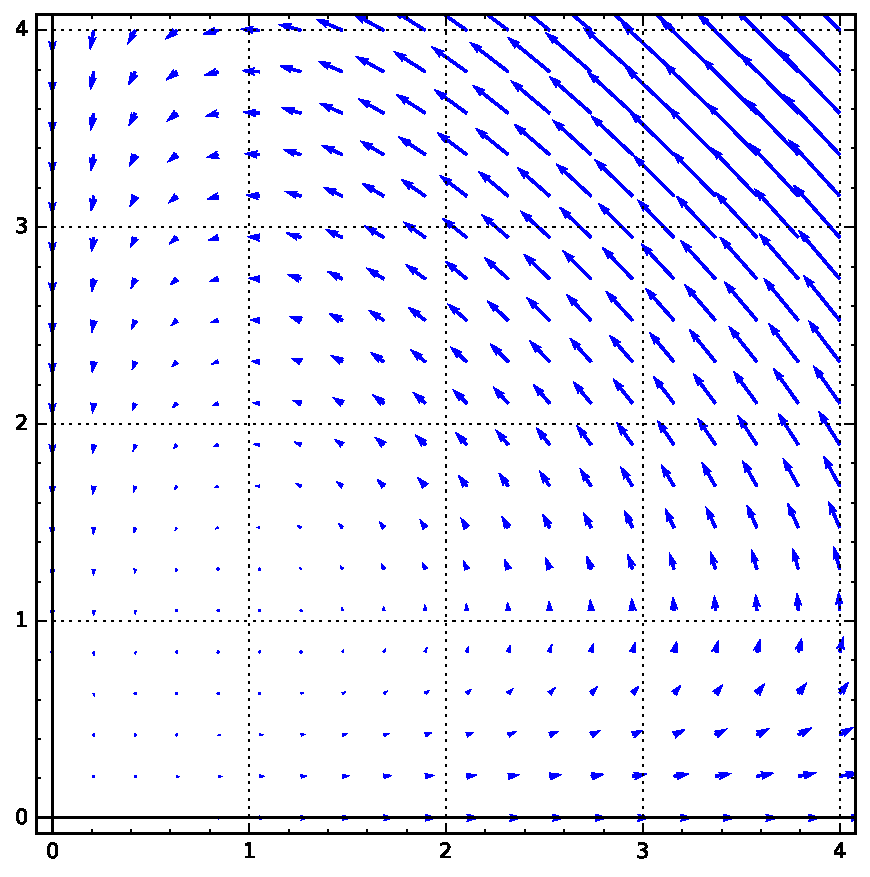
\includegraphics[width=0.46\textwidth]{2s_phase_plane}}}%
\quad
\subfloat[Normalized phase plane]{
    {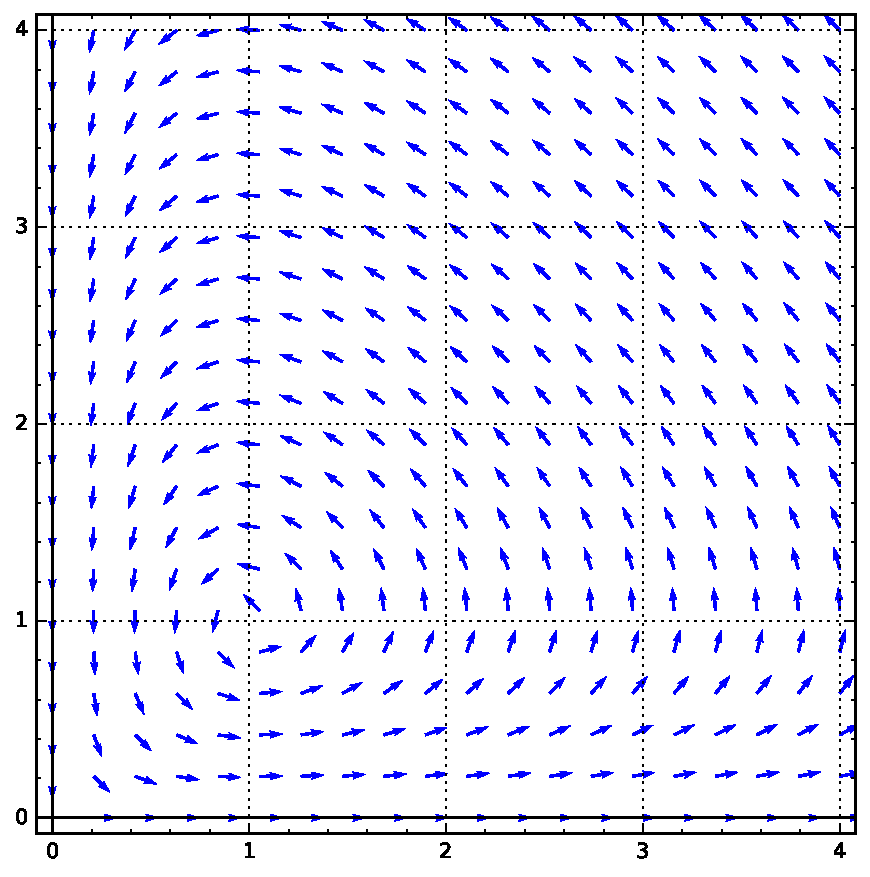
\includegraphics[width=0.46\textwidth]{2s_phase_plane_normalized}}}%
\caption{Two-species system phase planes with $a=b=c=d=1$}%
\label{fig:2s_phase_plane}%
\end{figure}
Part (\textsc{a}) gives insight into the speed of the system while the
normalized (same-length) vectors in part (\textsc{b}) give more insight into
the direction at a point. These two phase planes contain a lot of information
about the system \eqref{eq:2s_example}. We can see that \eqref{eq:2s_example}
moves faster as the distance to the origin increases and moves slowly around
the point $(1,1)$. Furthermore, the system moves counterclockwise around
a point approximately at $(1,1)$ at all distances from it. From
\autoref{sec:phase_plane} we know that a point that does not move in a phase
plane is a equilibrium, thus we can suspect that $(1,1)$ is an equilibrium of
this system. Additionally, the counterclockwise movement could represent closed
curves that are periodic solutions of \eqref{eq:2s_example}. 

The next graph in \figref{fig:2s_phase_plane_contours} shows a normalized phase
plane with contours. The contours are closed curves on the phase plane which
means that they are periodic solutions to system \eqref{eq:2s_example}. The
contours in this graph are generated using the family of equations 
\begin{equation}
    C = a \ln y - by + c \ln x - dx
\label{eq:2s_solution}
\end{equation}
($C$ being a constant) that, according to \cite{chauvet}, is a solution to
\eqref{eq:2s_system}. Using \eqref{eq:2s_solution} with the parameters
$a=b=c=d=1$, we can draw these contours to show some possible periodic
solutions of \eqref{eq:2s_example}.
\makefig{H}{0.9\textwidth}{2s_phase_plane_contours}{Two-species system phase
plane with normalized vectors, contour lines, and $a=b=c=d=1$}

We can say from the above figure that our prediction of periodic solutions
using the phase planes was correct (this is supported by \cite{chauvet},
\cite{hoppensteadt}, \cite{wangersky}). When it comes to $(1,1)$ as the
equilibrium of the system, \figref{fig:2s_phase_plane_contours} supports that
assumption. The vectors close to it seem to rotate around it and all the
contours revolve around it. The equilibrium of equation \eqref{eq:2s_system}
can be found by considering the parameters. The equilibrium is $(c/d, a/b)$
\cite{chauvet}, and because our example as $a=b=c=d=1$, our equilibrium point
is $(1,1)$. At this point the number of prey and predator are perfectly
balanced and never change. The example has another equilibrium, the point
$(0,0)$. At this point there are no predators or prey and thus nothing
changes.

In \figref{fig:2s_phase_plane_contours} we can see that at the coordinate axes
where $x=0$ or $y=0$ the vectors all point in the same direction along one of
the axes. At $x=0$ all the vectors point towards the $x$-axis. $x=0$ is
analogous to there being zero prey, meaning that the predators will have no
food. This will lead to exponential death seen in \figref{fig:2s_x_zero_graph}.
Taking the initial values of $x=0$ and $y=3$ and numerically solving
\eqref{eq:2s_example}, we can draw that figure.
\makefig{H}{0.85\textwidth}{2s_x_zero_graph}{Two-species
system graph for $x=0$, $y=3$, and $a=b=c=d=1$}

At $y=0$ all the vectors point along the $x$-axis towards positive infinity.
This case is analogous to a system with no predators so the prey will multiply
unhindered and exponentially. In \figref{fig:2s_y_zero_graph} we see
a numerical solution to this system with $x=6$ and $y=0$ as initial conditions. 
\makefig{h}{0.8\textwidth}{2s_y_zero_graph}{Two-species system graph for $x=6$,
$y=0$, and $a=b=c=d=1$}

If neither $x$ nor $y$ are 0, this system has a periodic solution that can be
numerically or analytically found. Taking the initial conditions $x=6$ and
$y=3$ and graphing the result as a contour on a phase plane we get
\figref{fig:2s_contour}. If the same result is graphed over time with both
species' populations represented on the $y$-axis we get \figref{fig:2s_graph}.
This figure shows that $x$ and $y$ continuously oscillate, with the prey
population $x$ peaking before the $y$ population of predators. The reason for
that is that if the prey is numerous, the predators have more to eat and their
population grows. Then they eat more prey and reduce its numbers faster than
they can multiply. The number of prey goes down and then the predators don't
have enough food and their population shrinks. Then the prey population begins
to grow again. This cycle repeats and the predators always lag behind the prey.
Additionally, the cycles of predators and prey have the same period
\cite{chauvet}.
\makefig{h}{0.65\textwidth}{2s_contour}{Two-species
system contour for $x=6$, $y=3$, and $a=b=c=d=1$}
\makefig{h}{0.7\textwidth}{2s_graph}{Two-species system
graph for $x=6$, $y=3$, and $a=b=c=d=1$}

%==============================================================================

\section{Three-Species Food Chain}

A three-species food chain from equation \eqref{eq:3s_system} is a system that 
also has one prey with an infinite food supply, called $x$. This prey is being
preyed on by intermediate predator $y$ who exclusively eats $x$. Finally, apex
predator $z$ preys exclusively on $y$. Again, for this example we chose the 
parameters $a=b=c=d=e=f=g=1$ because it is simpler. System \eqref{eq:3s_system}
now becomes
\begin{equation}
    \left\{\begin{aligned}
        &\frac{dx}{dt} = x(1 - y)              &\text{Prey}\\
        &\frac{dy}{dt} = y(x - z - 1) \qquad &\text{Intermediate Predator}\\
        &\frac{dz}{dt} = z(y - 1)             &\text{Apex Predator}
    \end{aligned}\right.
    \label{eq:3s_example}
\end{equation}
Because we are now dealing with 3 species we can no longer use the phase planes
that were so helpful for the two-species food chain. Now our system exists in
3 dimensions so it is a good start to look at the coordinate planes first 
(following \cite{chauvet}). The following examples are based on the initial
conditions $x=6$, $y=3$, and $z=1$.

If $z=0$ ($xy$-plane), equation \eqref{eq:3s_example} becomes the same system
as the example for two-species food chains in \eqref{eq:2s_example}.
\begin{equation}\nonumber
    \left\{\begin{aligned}
        &\frac{dx}{dt} = x(1 - y)              &\text{Prey}\\
        &\frac{dy}{dt} = y(x - 0 - 1) = y(x-1) 
            \qquad &\text{Intermediate Predator}\\
        &\frac{dz}{dt} = 0(y - 1) = 0             &\text{Apex Predator}
    \end{aligned}\right.
\end{equation}
Using numerical solving to find the solution to the three-species system in
\eqref{eq:3s_example} with the initial conditions $x=6$, $y=3$, and $z=0$
yields the same system as can be seen in \figref{fig:2s_graph} which is
identical to \figref{fig:3s_z_zero_graph} below. \figref{fig:3s_z_zero_contour}
shows the contour of the current system in three dimensions where it just lays
in the $xy$-plane. This contour looks the same as the one obtained from the
two-species equation in \figref{fig:2s_contour}, further supporting their
sameness.
\makefig{H}{0.7\textwidth}{3s_z_zero_contour}{Three-species system contour for
$x=6$, $y=3$, $z=0$, $a=b=c=d=e=f=g=1$}
\makefig{H}{0.7\textwidth}{3s_z_zero_graph}{Three-species system graph for
$x=6$, $y=3$, $z=0$, $a=b=c=d=e=f=g=1$}

The second coordinate plane is the $zy$-plane. Here $x=0$ and thus intermediate
predator $y$ has so source of food and starves. Because $y$ starves $z$ will
also eventually starve because their food runs out. In the equation below all
factors of $y$ are negative meaning that it will always decline. Accordingly,
$z$ will also decline.
\begin{equation}\nonumber
    \left\{\begin{aligned}
        &\frac{dx}{dt} = 0(1 - y) = 0              &\text{Prey}\\
        &\frac{dy}{dt} = y(0 - z - 1)=y(-z-1) 
            \qquad &\text{Intermediate Predator}\\
        &\frac{dz}{dt} = z(y - 1)             &\text{Apex Predator}
    \end{aligned}\right.
\end{equation}
The population of $y$ will start dropping exponentially immediately because of
the lack of food but $z$ may rise for a bit because they can prey on $y$ until
$y$ dies out. The end result will be that all species eventually die out
because neither of them have sustainable food sources. Taking $x=0$, $y=3$, and
$z=1$ and solving \eqref{eq:3s_example} numerically yields
\figref{fig:3s_x_zero_graph}.
\makefig{h}{\textwidth}{3s_x_zero_graph}{Three-species system graph for
$x=0$, $y=3$, $z=1$, $a=b=c=d=e=f=g=1$}

The third coordinate plane is the $xz$-plane where $y=0$. In this plane the
intermediate predator $y$ does not exist and thus $z$ always exponentially
declines and starves because of lack of food. On the other hand, $x$ is now
free from predation and will exponentially grow in population size. 
\begin{equation}\nonumber
    \left\{\begin{aligned}
        &\frac{dx}{dt} = x(1 - 0) = x              &\text{Prey}\\
        &\frac{dy}{dt} = 0(x - z - 1)=0 \qquad &\text{Intermediate Predator}\\
        &\frac{dz}{dt} = z(0 - 1) = -z             &\text{Apex Predator}
    \end{aligned}\right.
\end{equation}
This system results in a exponentially and unboundedly growing prey population
and a exponentially declining apex predator population that will die out. This
results in only species $x$ surviving.
\makefig{h}{\textwidth}{3s_y_zero_graph}{Three-species system graph for
$x=6$, $y=0$, $z=1$, $a=b=c=d=e=f=g=1$}

\newpage
All coordinate planes of this system are invariant, meaning a system never
escapes from a coordinate plane. This makes sense because on a coordinate plane
one species does not exist and it cannot just come back \cite{chauvet}. One
point of this system that is obvious is $(0,0,0)$ where it never changes and
thus has a equilibrium. When it comes to the coordinate axes, two of the values
must be zero. As established above, if $x=0$ all species eventually die out.
This means that for the $y$- and $z$-axis both species will eventually die out.
If our system starts on the $x$-axis species $x$ will grow unboundedly and the
other species will remain at 0.

In their analysis in \cite{chauvet} the authors use further criteria to
analyze system \eqref{eq:3s_system}. They use the equations and inequalities
below to describe the systems' behaviors not already mentioned. These
classifications are purely based on the constants $a,b,f,g$ \cite{chauvet}
\begin{equation}\nonumber
    ga > fb, \qquad ga < gb, \qquad  ga = fb.
\end{equation}
If $ga > fb$, for example $a=g=1.1$ and all other constants equal to 1, 
equation \eqref{eq:3s_system} becomes
\begin{equation}\nonumber
    \left\{\begin{aligned}
        &\frac{dx}{dt} = 1.1x - xy              &\text{Prey,}\\
        &\frac{dy}{dt} = -y + xy - yz \quad &\text{Intermediate Predator,}\\
        &\frac{dz}{dt} = -z + 1.1yz             &\text{Apex Predator.}
    \end{aligned}\right.
\end{equation}
This equation suggests that species $x$ is now growing quicker than before
while the predation by $y$ has remained the same. The change of species $y$
remain unchanged and species $z$ now grows more from eating species $y$ than
before. All these observations combined would suggest that the populations of
both $x$ and $z$ increase over time while $y$ could remain the same. When the
above equation is numerically solved for the mentioned constants and the
initial conditions $x=6$, $y=3$, and $z=1$ and then graphed
\figref{fig:3s_ga_g_fb_graph} is created.
\makefig{h}{\textwidth}{3s_ga_g_fb_graph}{Three-species system graph for
$x=6$, $y=3$, $z=1$, $b=c=d=e=f=1$, and $a=g=1.1$}

This graph confirms the prediction as it shows that $z$ and especially $x$
increase over time but that $y$ remains the same. The analysis in
\cite{chauvet} showed that the populations of both $x$ and $z$ approach
infinity, but not monotonically because of the oscillations. For $y$ the peaks
will become taller and skinnier but at a much slower rate. Overall, no species
will die out and two of them will increase without bound.

If $ga < fb$, e.g. $b=f=1.1$ and all other constant equal 1, the general
three-species system \eqref{eq:3s_system} turns into
\begin{equation}\nonumber
    \left\{\begin{aligned}
        &\frac{dx}{dt} = x - 1.1xy              &\text{Prey,}\\
        &\frac{dy}{dt} = -y + xy - yz \quad &\text{Intermediate Predator,}\\
        &\frac{dz}{dt} = -1.1z + yz             &\text{Apex Predator.}
    \end{aligned}\right.
\end{equation}
The system above suggests that now the predation effect of $y$ on $x$ will be
stronger and that the natural death rate of $z$ increased. The increase in
death rate of $z$ could lead to a drastic reduction in population size or even
extinction while the increased effect of predation of $y$ on $x$ might decrease
the population size of $x$ and subsequently of $y$ because there is now less
prey. \figref{fig:3s_ga_l_fb_graph} is the result of numerical solving of
\eqref{eq:3s_system} with the above mentioned constants and the initial
conditions $x=6$, $y=3$, $z=1$.
\makefig{h}{\textwidth}{3s_ga_l_fb_graph}{Three-species system graph for
$x=6$, $y=3$, $z=1$, $a=c=d=e=g=1$, and $b=f=1.1$}
The figure supports the hypothesis that $z$ might go extinct and in fact shows
that that happens. As expected, the increased predation effect of $y$ on $x$
causes its population to shrink and then subsequently to make the population of
$y$ shrink. When $z$ goes extinct the system has been reduced to a two-species
system of equations as in \eqref{eq:2s_system}. This system will then
periodically oscillate like a normal two-species food chain. In
\figref{fig:3s_ga_l_fb_contour} the three-dimensional contour of the system is
shows and one can see that the system spirals downwards towards the $xy$-plane.
\makefig{h}{0.8\textwidth}{3s_ga_l_fb_contour}{Three-species system contour for
$x=6$, $y=3$, $z=1$, $a=c=d=e=g=1$, and $b=f=1.1$}
\newpage

The last of the three options is that $ga = fb$. In this case we can keep our
simple setup of $a=b=c=d=e=f=g=1$ and the original example equation 
\eqref{eq:3s_example} does not change. In this particular system all the
constants are equal so one could maybe expect the system to oscillate
indefinitely like a two-species system. Using numerical solving and the initial
conditions $x=6$, $y=3$, and $z=1$ we get the graph in
\figref{fig:3s_ga_eq_fb_graph}. 

In said figure we see three continuously oscillating graphs that have the same
period. The highest peaks are the prey $x$, followed by intermediate predator
$y$ and then by apex predator $z$. The peaks are also shifted in time, with the
graphs lagging behind each other in the same fashion, first $x$, then $y$, and
then $z$. This has the same cause as the lag in the two-species system -- it
takes the species a while to react to increased or decreased numbers of
predators and prey. In this system no species dies out and they all continue to
exist. \figref{fig:3s_ga_eq_fb_contour} shows the contour of this system in
three-dimensional space where it looks similar to a contour in two-dimensional
space.
\makefig{h}{0.8\textwidth}{3s_ga_eq_fb_graph}{Three-species system graph for
$x=6$, $y=3$, $z=1$, and $a=b=c=d=e=f=g=1$}
\makefig{h}{0.5\textwidth}{3s_ga_eq_fb_contour}{Three-species system contour for
$x=6$, $y=3$, $z=1$, and $a=b=c=d=e=f=g=1$}

%==============================================================================

\section{Conclusion}
The systems covered in this report are models for two and three-species food
chains. As models, they fit most of the intuitions one has about what 
should happen to biological systems in certain situations. If there are no
predators, they prey multiply greatly; if there is no prey the predators
starve. 

Some inaccuracies of these models are the restricted behavior of predator and
prey when they only live off one thing and the fact that the prey has an
infinite supply of food. Another aspect is the exponential and unbounded growth
of prey populations if there are no predators. In many more accurate and
complicated systems use logistic equations to get around this issue and make
the equations more accurate. 

To conclude, the two and three-species models covered in this report are
relatively accurate in spite of their simplicity and can be analyzed using
numerical solution methods and, for the two-species model, phase planes. The
Lotka-Volterra equations \eqref{eq:2s_system} had a great impact on biology and
ecology \cite{wangersky} and can, especially with modifications, still be 
relevant today.

\bibliography{../bibliography}
\bibliographystyle{siam}

\end{document}
